\begin{figure}[!h]
	\centering
	\subbottom[before adjustment\label{fig:egadj0}]
		{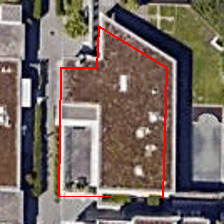
\includegraphics[width=0.243\textwidth]{4-04-0.png}}
	\subbottom[before adjustment\label{fig:egadj1}]
		{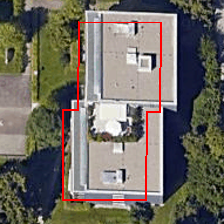
\includegraphics[width=0.243\textwidth]{4-04-1.png}}
	\subbottom[before adjustment\label{fig:egadj2}]
		{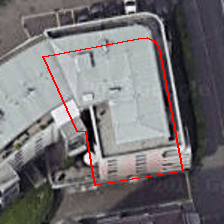
\includegraphics[width=0.243\textwidth]{4-04-2.png}}
	\subbottom[before adjustment\label{fig:egadj3}]
		{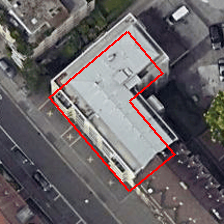
\includegraphics[width=0.243\textwidth]{4-04-3.png}}
	\subbottom[after adjustment\label{fig:egadj4}]
		{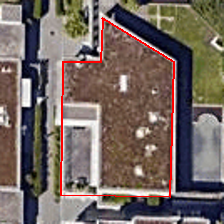
\includegraphics[width=0.243\textwidth]{4-04-4.png}}
	\subbottom[after adjustment\label{fig:egadj5}]
		{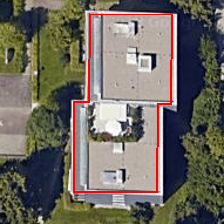
\includegraphics[width=0.243\textwidth]{4-04-5.png}}
	\subbottom[after adjustment\label{fig:egadj6}]
		{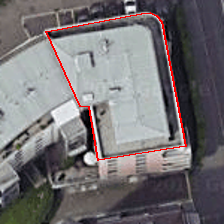
\includegraphics[width=0.243\textwidth]{4-04-6.png}}
	\subbottom[after adjustment\label{fig:egadj7}]
		{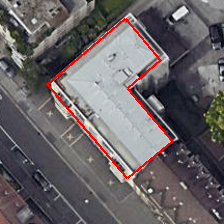
\includegraphics[width=0.243\textwidth]{4-04-7.png}}
    \caption{Adjustment examples. (a)--(d) show the polygon before adjustment, while (e)--(h) show the polygon after adjustment.}
	\label{fig:egadj}
\end{figure}